\chapter{The GEM Data Acquisition System}
\label{chap:II-2-daq}

  The installation of GEM detectors in CMS and the integration with the CSCs require the development of a new DAQ system for the GE1/1 project. The understanding of the structure of both the GEM readout chain as well as the common CMS DAQ is of importance in the scope of this thesis. To this end, these systems are presented in details in the sections that follow. \\

  \section{The GE1/1 Data Acquisition System}

    The architecture of the GE1/1 DAQ system is represented in Figure \ref{fig:II-2-daq-gem-system}. It is divided into two sectors: the on-detector electronics on the left in charge of the managment of the detector, and the off-detector electronics on the right responsable for the data handling and the connection to the central DAQ. The two sectors are separated by a few dozen meters and connected through optical fibres. \\

    \begin{figure}[h!]
      \centering
      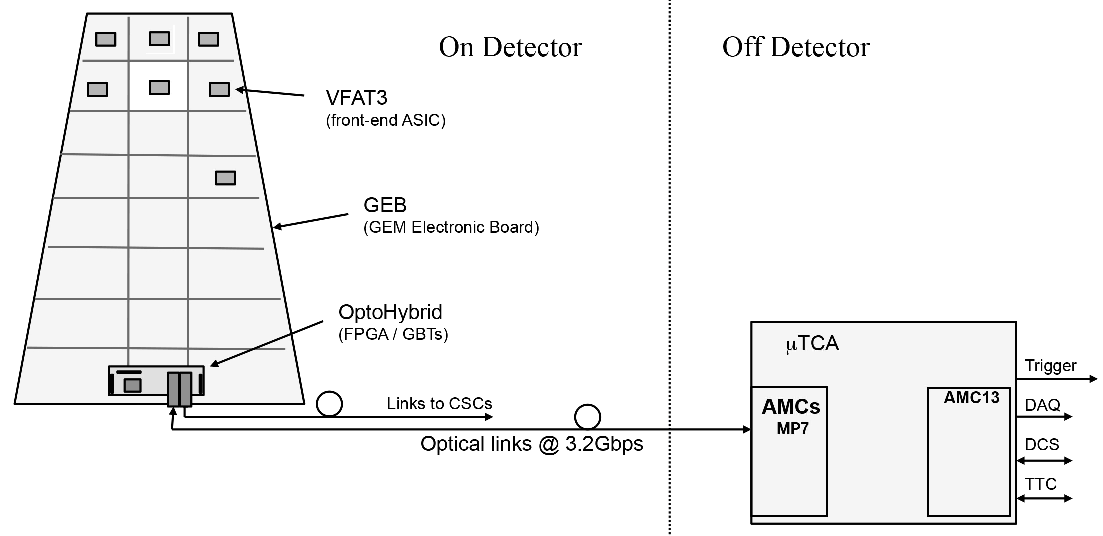
\includegraphics[width=0.9\textwidth]{img/II-2-daq/gem-system.pdf}
      \caption{??? \cite{Colaleo:2021453}.}
      \label{fig:II-2-daq-gem-system}
    \end{figure}

    The on-detector electronics focuses on the control and readout of the VFAT3 Application Specific Integrated Circuit (ASIC) which connects to the strips of the chamber and digitizes the data. The GEM Electronic Board (GEB), on which the VFAT3s are plugged in, then routes the signals to the OptoHybrid which acts as concentrator board and communication relay for the 24 VFAT3s. The communication with the off-detector system is performed through the GigaBit Tranciever (GBT) chipset and the Versatil Link installed on the OptoHybrid. Both projects are led by CERN and provide radiation hard tools for LHC experiments. \\

    On the off-detector side, the Micro Telecommunications Computing Architecture (microTCA, MTCA, or $\mu$TCA) \cite{PICMG} crate standard is used to power and monitor the Advanced Mezzanine Cards (AMCs) which provide the ressources to communicate with the on-detector electronics. Links from multiple OptoHybrids are concentrated on one MP7 AMC which formats the data and transfers it to the CMS AMC13 mezzanine. The AMC13 is the link between the microTCA crate and the central DAQ of CMS which provides the clocking, trigger, and control over the system. The control of the DAQ chain is performed from a XDAQ application using the IPBus protocol over ethernet.

    \subsection{The VFAT3 ASIC}

      The VFAT3 ASIC is a binary front-end chip optimized for gaseous detectors which function is to digitize the analog signals coming from the detector and provide fast trigger and tracking data. The trigger data is sent at the LHC clock over a fixed latency path and then used in the algorithms of the L1 trigger to accept or reject events. The tracking data holds the full granularity information of the events that have been accepted and follows a variable latency path. The logic diagram of the chip is shown in Figure \ref{fig:II-2-daq-vfat3}. It is made of an analog front-end which amplifies, shapes, and digitizes the signal from the GEM strips, and of a digital back-end for slow control, fast control, and data readout. \\

      \begin{figure}[h!]
        \centering
        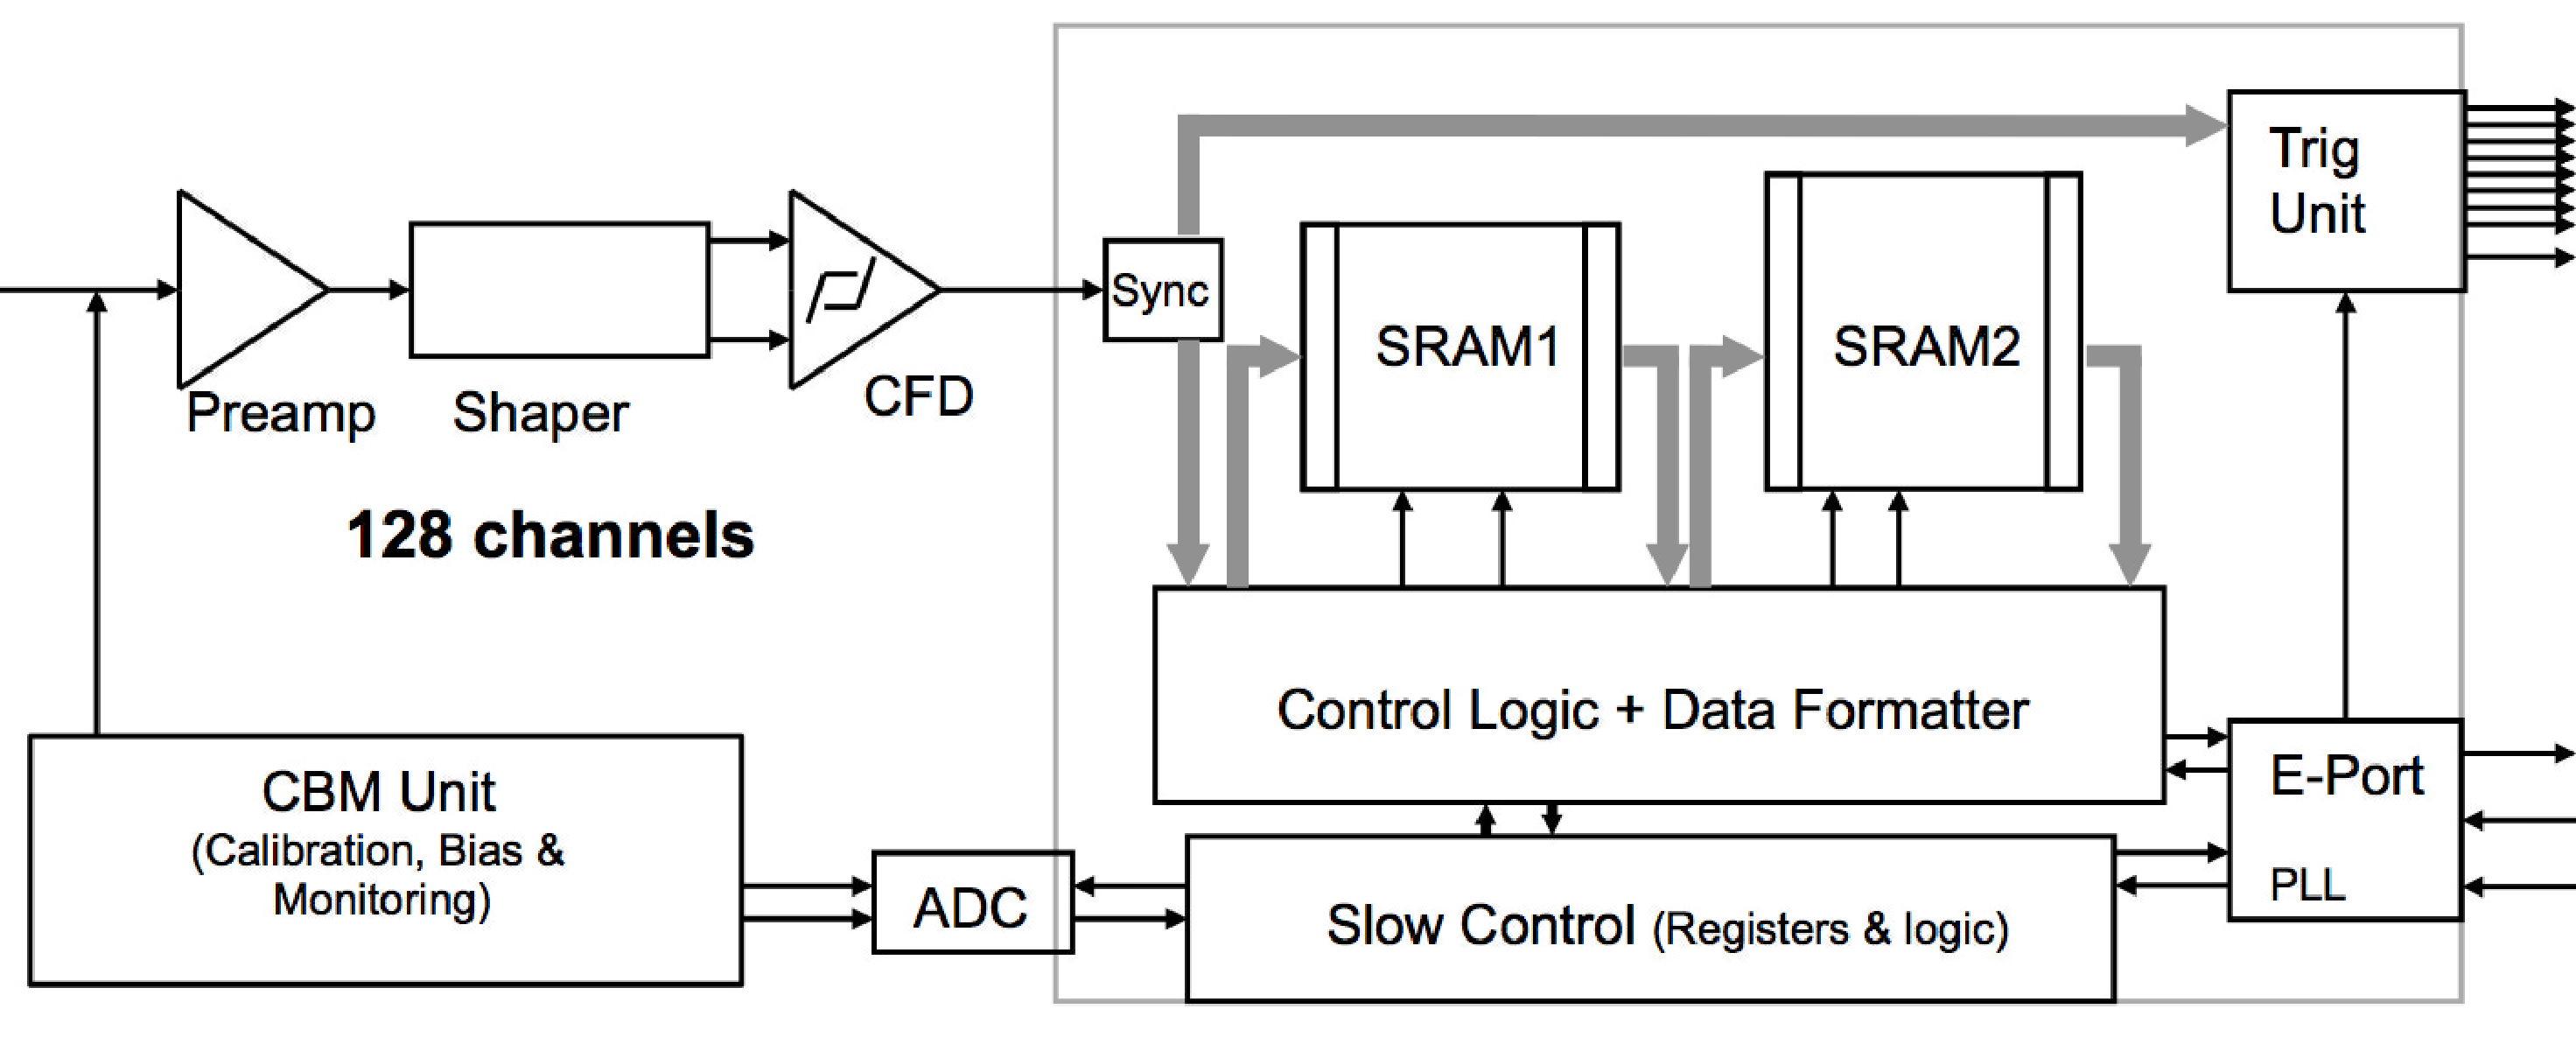
\includegraphics[width=\textwidth]{img/II-2-daq/vfat3.pdf}
        \caption{??? \cite{Colaleo:2021453}.}
        \label{fig:II-2-daq-vfat3}
      \end{figure}

      \paragraph{The analog front-end} is further optimized for the readout of GEMs in particular. It is composed of 128 channels which amplify and shape the analog signals from the strips with programmable shaping times to allow for various integration lengths of the signal. According to the gas mixture, signal charge from the GEM can last for approximatly 60 ns. Increasing the shaping time to fully integrate the charge will result in a higher signal to noise ratio. Simulations performed on the analog front-end show that a time resolution of 7 ns can be achieved by using a Constant Fraction Discriminator (CFD) with a shaping time of 50 ns. After shaping, the amplitude of the analog signal is compared against a programmable threshold by a comparator to yield a binary output flag for each channel. \\

      \paragraph{The fixed latency path} is used to provide a fast hit information to the trigger system of CMS at a frequency equal to the LHC clock of 40 MHz. The trigger unit inside the VFAT3 formats the output of the 128 comparators and transmits it over 8 differential pairs at a rate of 64 bits per BX. It allows to either encode a logical-OR of two adjacent strips effectivly dividing the number of bits to send by a factor two, or use a zero supression algorithm to solely transmit information on hit strips. Ensuring a fixed latency on this path in crucial to maintain predictability in the trigger system and identify the correct BX. \\

      \paragraph{The variable latency path} is activated upon reception of an L1A to transmit the full granularity information on an event that has been accepted by the trigger system. The VFAT3 holds two Static Random-Access Memories (SRAMs) which are used to store events. The SRAM1 is a circular buffer filled at a frequency equal to the LHC clock with the output of the 128 comparators. When the VFAT3 receives an L1A, it transfers a given event from the SRAM1 to the SRAM2 and adds the BX Counter (BC) and the Event Counter (EC), which respectivly count the number of BX elapsed and the number of L1A received, to the event data. To determine which event needs to be transfered, the chip uses a programmable parameter called the latency that informs the system on the delay between the digitization of an event and the arrival of an L1A corresponding to the same event. It is a measures of the response time of the trigger system to a given event which is a fixed delay. Events stored in the SRAM2 are then formated and sent over a single differential pair out of the VFAT3. The formatting of the data can be selected using a programmable register to be either lossless or zero suppressed. \\

      \paragraph{The slow control} module handles the configuration of the internal registers of the VFAT3. These registers define quantities such as the threshold of the analog front-end, the latency, the readout data format, etc. Coupled with the Calibration, Bias \& Monitoring (CBM) unit, it allows to perform calibration routines on the chip. \\

      \paragraph{The fast control} defines all the time sensitive commands that the VFAT3 receives. These are the Event Counter 0 (EC0), Bunch Counter 0 (BC0), Calibration Pulse (CalPulse), Resynchronisation (Resync), and L1A. The EC0 and BC0 commands respectivly reset the EC and BC; the CalPulse is used to send a calibration pulse on given strips in order to callibrate the analog front-end; the ReSync command resets the internal pointers; and the L1A informs the VFAT3 that an event needs to be transfered to the DAQ.

    \subsection{The GEM Electronic Board}

      The limited space in which the GEM detectors will be installed constrains the design of the system by making it impossible to run flat cables for the 24 VFAT3s. Therefore, the GEB, a Printed Circuit Board (PCB) of the same dimension as the GEM detector, was designed to route the signals of the front-end chips to the OptoHybrid located on the large side of the detector, furthest away from the beam pipe. A picture of a prototype of the GEB is shown on the right in Figure \ref{fig:II-2-daq-geb}. The functions of the GEBs are to host the VFAT3 ASICs connected to the 24 sectors of the GEM readout board, route their signals to the OptoHybrid, distribute power to the chips, and provide electric shielding to the detector. The GEB is divided into three columns of eight VFAT3s, further divided into two sectors each as represented in the left picture in Figure \ref{fig:II-2-daq-geb}. The clock, slow control, and fast control are commonn for each column. \\

      \begin{figure}[h!]
        \centering
        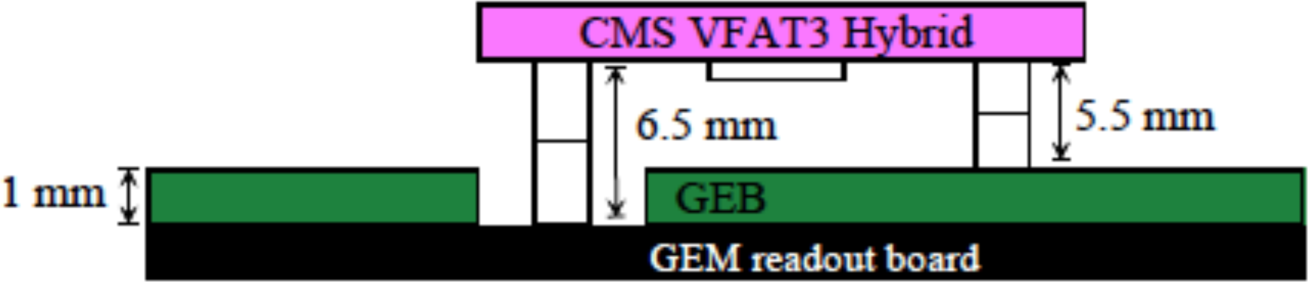
\includegraphics[width=0.8\textwidth]{img/II-2-daq/geb.pdf}
        \caption{??? \cite{Colaleo:2021453}.}
        \label{fig:II-2-daq-geb}
      \end{figure}

      The VFAT3s are soldered on the GEB and connected to the GEM readout board on which it rests through a flexible PCB. The control and data signals from the chips are routed on the PCB towards four connectors located on the large side of the detector which connect to the OptoHybrid. The power for the VFAT3s and the OptoHybrid is distributed by the GEB using radition hard DC/DC converters developped by CERN which convert the incoming low voltage to the required voltages. In addition, the bottom layer of the GEB is grouded proving shielding to the detector from external ElectroMagnetic Interference (EMI).

    \subsection{The OptoHybrid}

      The OptoHybrid is the interface between the VFAT3 ASICs and the off-detector system. It is a 10 cm $ \times $ 20 cm board mounted on the GEB equipped with a Field Programmable Gate Array (FPGA) and Integrated Circuits (ICs) dedicated to the operation of the optical links. The FPGA solely handles the trigger data by applying zero suppression algorithms, formatting the data, and sending it to the CSC and the GEM trigger system separatly over two optical links using the SFP+ connectors. The other functions of the VFAT3s are directly connected to the three GBT chipsets installed on the OptoHybrid. Each GBT chipset is capable of handling a column of eight VFAT3s.

    \subsection{The GBT and Versatil Link}

      The GBT \cite{Moreira:1235836} and Versatil Link \cite{Soos:1609037} are projects developped by CERN providing radiation hard tools for optical communication to the LHC experiments. The GBT is an optical data link technology providing bidirectionnal 4.8 Gb/s (Gigabits per second) serial communication designed to connect the on-detector and off-detector electronics. It is declined in two version: the GBTX which is a radiation hard ASIC, and the GBT-FPGA which is a core that can be implemented inside an FPGA. Complementary to the GBT which provides the data structure and communication protocol between components, the Versatil Link project develops radiation hard optical transceivers. The integration of the GBTX, Verstil Link, and GBT-FPGA projects is shown in Figure \ref{fig:II-2-daq-gbt-versatile}. \\

      \begin{figure}[h!]
        \centering
        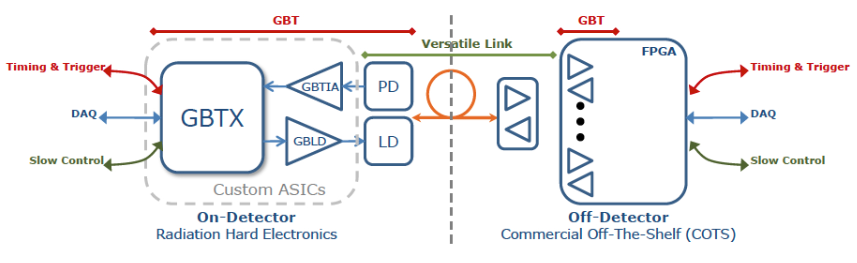
\includegraphics[width=\textwidth]{img/II-2-daq/gbt-versatile.pdf}
        \caption{??? \cite{Moreira:1235836}.}
        \label{fig:II-2-daq-gbt-versatile}
      \end{figure}

      The GBT defines a data format shown in Figure \ref{fig:II-2-daq-gbt-frame}. The stream of data is divided into frames of 120 bits transmitted at 40 MHz, resulting in a data rate of 4.8 Gb/s from which 3.36 Gb/s are accessible by the user. The frame start with a four bits header (H) which defines the frame type and ends with 32 bits of Forward Error Correction (FEC). The error correction is done by encodeding the data using a Reed-Salomon code that can correct bit flips due to radiation. The 84 remaining bits are user accessible. The first two bits are used for internal slow control (IC) and the two following bits for external slow control (EC), leaving 80 bits of data (D) accessible to the user for DAQ, TTC, and slow control purposes. \\

      \begin{figure}[h!]
        \centering
        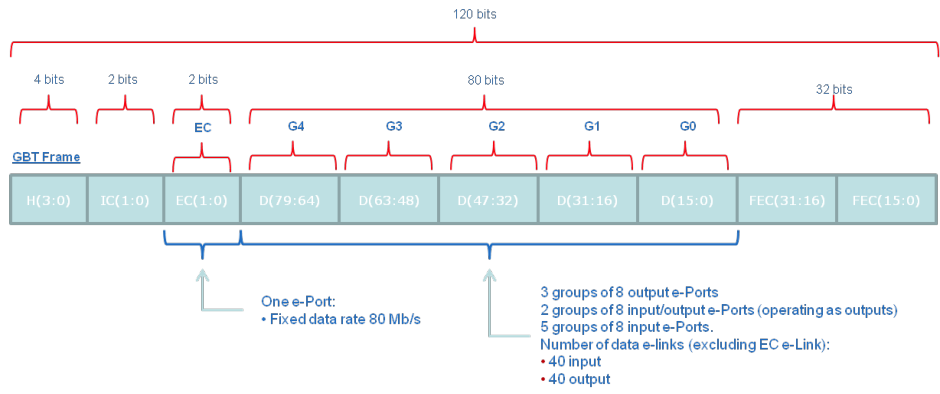
\includegraphics[width=\textwidth]{img/II-2-daq/gbt-frame.pdf}
        \caption{??? \cite{Moreira:1235836}.}
        \label{fig:II-2-daq-gbt-frame}
      \end{figure}

      The header is used to syncrhonize the link by requiering the detection of a series of valid header fields. It is therefore protected by the FEC in order to ensure efficient frame-locking. From the slow control bits, both running at 80 Mb/s, the IC is reserved for the control and monitoring of the GBTX while the EC on the other hand can be freely assigned by the user. The data field is used to transfer DAQ, TTC, and slow control requests to the various subsystems connected to the GBT and can implement any user defined protocol. The FEC uses two Reed-Salomon codes interleaved with 4-bit symbols each capable of correcting double errors. This means that the total frame can recover up to 16 corrupted bits. Additionnaly, the GBT frame is scrambled in order to maintain DC balance on the transmission lines. \\

      On the FPGA side, the communication protocol is seen by the user as a 84-bits-wide vector that is sampled at a frequency of 40 MHz an then formatted by the GBT-FPGA core. The GBTX ASIC on the other hand uses 42 Electric serial Links (E-Links) to handle the data. The structure of the GBTX is shown in Figure \ref{fig:II-2-daq-gbt-asic}. Each E-Link is composed of three differential pairs: one to transmit and one to receive the data, and one to carry the clock synchronuous to the data. From the 42 E-links, one is dedicated to the IC and one to the EC, each transfering data at 80 Mb/s by serializing the two IC or EC bits of the GBT frame on a single link. The use of the remaining 40 E-Links is defined according to the speed at which they operate. The 80-bit-long user data can be configured to either be serialised by a factor two, four, or eight resuling in the use of 40, 20, or 10 E-Links respectivly running at 80 MHz, 160 MHz, or 320 MHz to accomodate the data rate. For the GEM project, a serialisation factor of eight is used, meaning that from the 40 E-Links, only 10 are in used, each of them tranfering 8 bits per BX. \\

      \begin{figure}[h!]
        \centering
        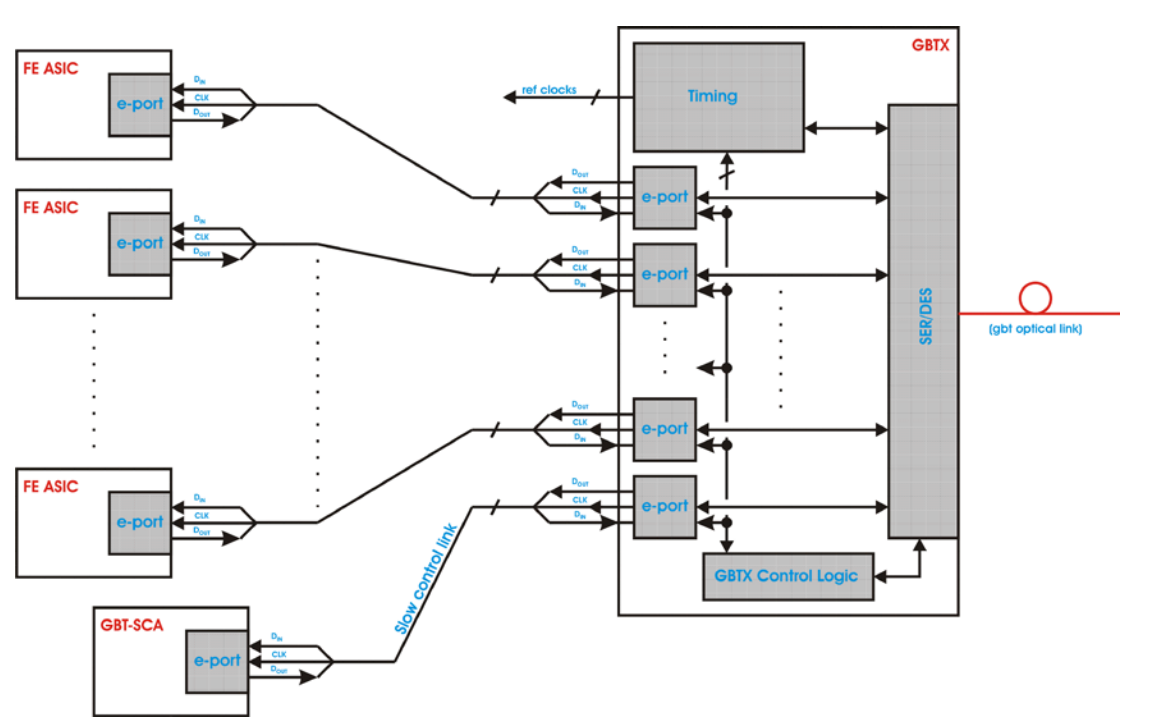
\includegraphics[width=0.8\textwidth]{img/II-2-daq/gbt-asic.png}
        \caption{??? \cite{Moreira:1235836}.}
        \label{fig:II-2-daq-gbt-asic}
      \end{figure}

      To convert the GBTX signals into optical communication, the Versatil Link project provides two laser diode modules: a transceiver module called VTRx and a dual transmitter module called VTTx. The modules have been designed to wistand high magnetic field and radiation doses as encountered in the LHC experiments. The maximal bit rate is of 4.8 Gb/s with a bit error rate inferior to 10$^{-12}$.

    \subsection{The microTCA Standard}

      The off-detector electronics is implemented using the microTCA crate standard to manage the back-end system. The microTCA standard was developped for the telecommunication industry as a successor for the Advanced Telecommunications Computing Architecture (ATCA) technology. It uses a smaller form factor for the AMCs declines into a single width (73.8 mm $ \times $ 181.5 mm) or double width (148.8 mm $ \times $ 181.5 mm) version. The key feature of the crate is the topology of the backplane connecting the AMCs. The latter is not defined in the specifications but often implements a dual-star network which provides reduduncy and thus avoid critical failures of the system upon malfunction of a component. \\

      The structure of the crate is shown in Figure \ref{fig:II-2-daq-utca-crate}. Managment and control of the subsystems of the crate are performed by the MicroTCA Carrier Hub (MCH), which in failure critical systems can be accompagnied by a second MCH for redunduncy. These two MCHs are the central points of the network in dual-star topology. They communicate with the Cooling Units (CUs), Power Modules (PMs), and AMCs through the Intelligent Platform Management Interface (IPMI). The CUs and PMs are equipped with a Enhanced Module Managment Controller (EMMC) and the AMCs with a Module Managnment Controller (MMC) which are used to communicate with the MicroTCA Carrier Management Controller (MCMC) of the MHCs. These controllers implement the IPMI protocol and provide system managment functions to the crate. Upon power-on of the crate or hot-swap of an AMC, the MCHs provide minimal power to the EMMCs and MMCs through dedicated lines in order to start the initial transaction sequence. During this exchange, the power requirements of the modules are defined and a boot-up sequence takes place. Once the transaction is closed, power is provided to the rest of the module and normal operation begins. A power-off sequence takes place when the crate is shutdown or an AMC is removed. \\

      \begin{figure}[h!]
        \centering
        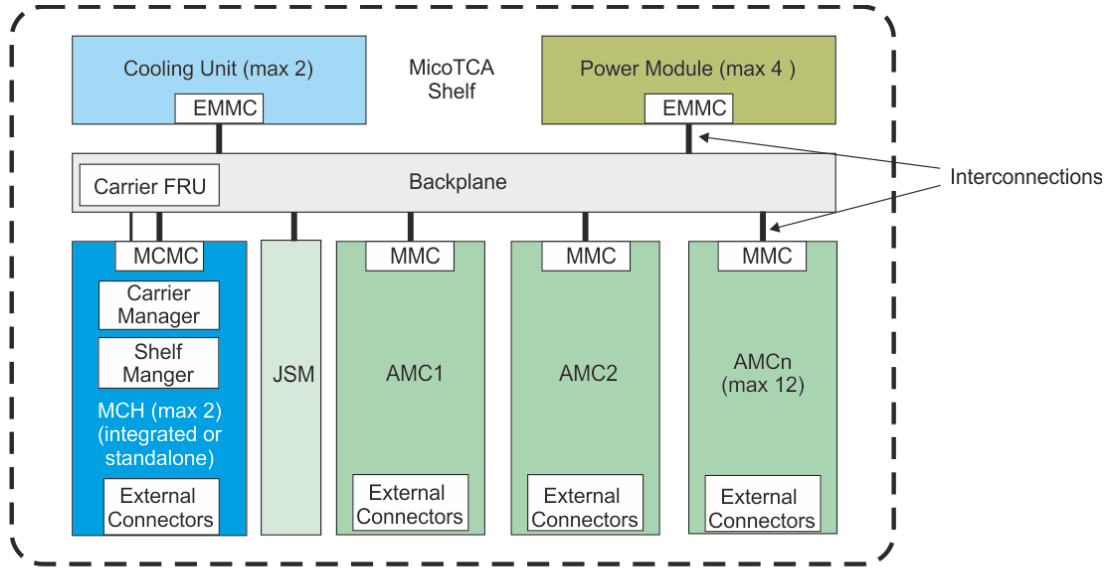
\includegraphics[width=\textwidth]{img/II-2-daq/utca-crate.png}
        \caption{??? \cite{VADATECH}.}
        \label{fig:II-2-daq-utca-crate}
      \end{figure}

      The backbone of the microTCA crate is its backplane. It provides point to point connections between the AMCs and MCH to AMC connections. The interconnects between elements are called fabrics and are what defines the topology of the crate. On the AMCs, the connections to the backplane are called ports. In the dual-star topology, each fabric is duplicated and connected to a separate MCH. As the backplane topology is not described in the specifications of the standard, a common topology is described.
      \begin{itemize}
        \item Fabric A is used for Gigabit Ethernet communication between the AMCs and MCH1 on port 0 and the MCH2 on port 1.
        \item Fabric B is allocated for technologies such as Seriel-ATA through port 2 and 3 for the MCH1 and MCH2 respectrivly.
        \item Fabric C is only used in single MCH mode and uses port 3 to connect the AMCs to MCH1.
        \item Fabric D to G are fat pipes which use multiple protocol agnostic links to connect the AMCs to the MCH1 on ports 4 to 7 and to the MCH2 on ports 8 to 11.
        \item Some backplanes implement point to point communication between ACMs on ports 12 to 20 following a custom interconnect.
      \end{itemize}
      Next to signal busses, the microTCA standard defines three clocks busses that can originate from the MCHs or the AMCs.

    \subsection{The MP7 Advanced Mezzanine Card}

      The AMC board used as back-end electronics is the MP7 \cite{MP7} developped by Imperial College and shown in Figure \ref{fig:II-2-daq-mp7}. It is equipped with a large Virtex-7 FPGA providing extensive computanionnal power. The optical interface with the on-detector electronics is done through six Avago MiniPOD transmitters and six Avago MiniPOD receivers for a total of 72 bidirectionnal links. Using one MP7, 9 superchambers can be readout thus requiering a total of 8 MP7s for the GE1/1 project. \\

      \begin{figure}[h!]
        \centering
        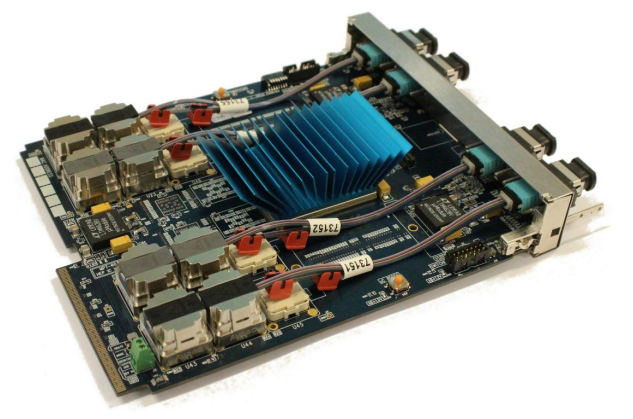
\includegraphics[width=0.8\textwidth]{img/II-2-daq/mp7.png}
        \caption{??? \cite{MP7}.}
        \label{fig:II-2-daq-mp7}
      \end{figure}

      The function of the MP7 is tripe: handle slow control requests for the subsystems, interpret TTC signals, and readout the trigger and tracking data from the OptoHybrids. The MP7 is the interface between the control and monitoring software and the detector electronics. It uses the fabric A lines of the MCH1 to connect to a Gigabit Ethernet network and handle TCP/IP requests. It interprets the requests and forwards them to the appropriate subsystem: either itself or over the optical link to the OptoHybrids and VFAT3s. The MP7 also receives the TTC commands on the fabric B from MCH2 and must forward them to the subsystems along with the LHC clock received on the CLK1 line. Finally, when the VFAT3s or the OptoHybrids push data upwards to the MP7, the latter must format the data before sending it on the backplane to a dedicated DAQ AMC.

    \subsection{The AMC13}

      The module which delivers the TTC signals and the LHC clock to the MP7s and retreaves the trigger and tracking data from the backplane is the AMC13 \cite{AMC13}. It is a board specifically designed for CMS which replaces the MCH2 is the microTCA crate. Its functionnal diagram is shown in Figure \ref{fig:II-2-daq-amc13}. It is equipped with two FPGAs: a powerfull Virtex-6 for data handling, and a smaller Spartan-6 for control and monitoring. The TTC signal is received through an optical link from which the LHC clock is extracted along with the TTC commands. The clock is forwared on the CLK1 line and the TTC commands are passed to the Spartan-6 FPGA which formats them on the fabric B lines at 80 MB/s. Being in the MCH2 slot, the AMC13 has direct access to all AMCs, which it uses to retreive tracking and trigger data over the fabric A ports running at 5 Gb/s. For development purposses, the AMC13 integrates internal TTC commands and LHC clock generators. \\

      \begin{figure}[h!]
        \centering
        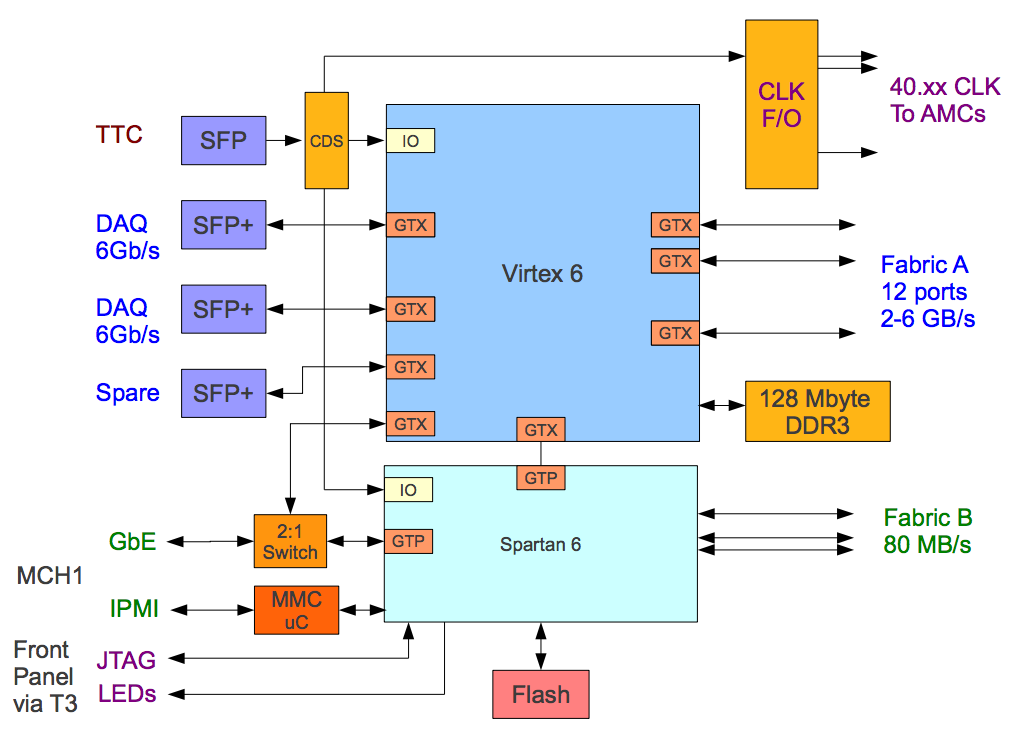
\includegraphics[width=\textwidth]{img/II-2-daq/amc13.png}
        \caption{??? \cite{AMC13}.}
        \label{fig:II-2-daq-amc13}
      \end{figure}

      The Virtex-6 FPGA of the AMC13 is connected to the central DAQ of CMS through the two SFP+ optical links running at 6 Gb/s which implement the S-Link Express protocol defined by CMS. An additionnal SFP+ can be used as spare if the bandwidth is required. Next to the data, the AMC13 also send TTS signals to the TCDS system to inform it about the status of the readout. The TTS codes can be: hardware failure, imminent overflow, sync lost, busy, ready, or error. Using these, the TCDS system can regulate the L1A rate for the system to be able to cope.

    \subsection{The IPBus Protocol}

      To communicate between the control and monitoring applications and the subsystems, a new protocol called IPBus has been developped for the CMS subdetectors. It uses the Internet Protocol (IP) and can be sent over User Data Protocal (UDP) or Transmission Control Protocol (TCP). IPBus transactions are simple read/write operations using a A32/D32 implementation (Address of 32 bits, Data of 32 bits). A sequence of transactions is called a packet which starts with a packet header of 32 bits which format is shown in Figure \ref{fig:II-2-daq-ipbus}. \\

      A transaction is always performed in two stages: a request from the applications is sent to which the system provides a response. The header of the request specifies the request type and request size. Additionnal 32 bits words are added in function of the type of operation to perform. For a read operation, the base address of the read must be specified. The response will contain N 32 bits words corresponding to the data at the base address and the incremental N addresses where N is the size of the request defined in the header. For a write operation, the request will contain the base address followed by N 32 bits words that should be written at the base address and the N following addresses where N is the size of the request defined in the header. The response will be a single header containing a status code. Variation of the read/write operations exist such as the FIFO-read and FIFO-write, which repeatevly read and write words at the same address. \\

      \begin{figure}[h!]
        \centering
        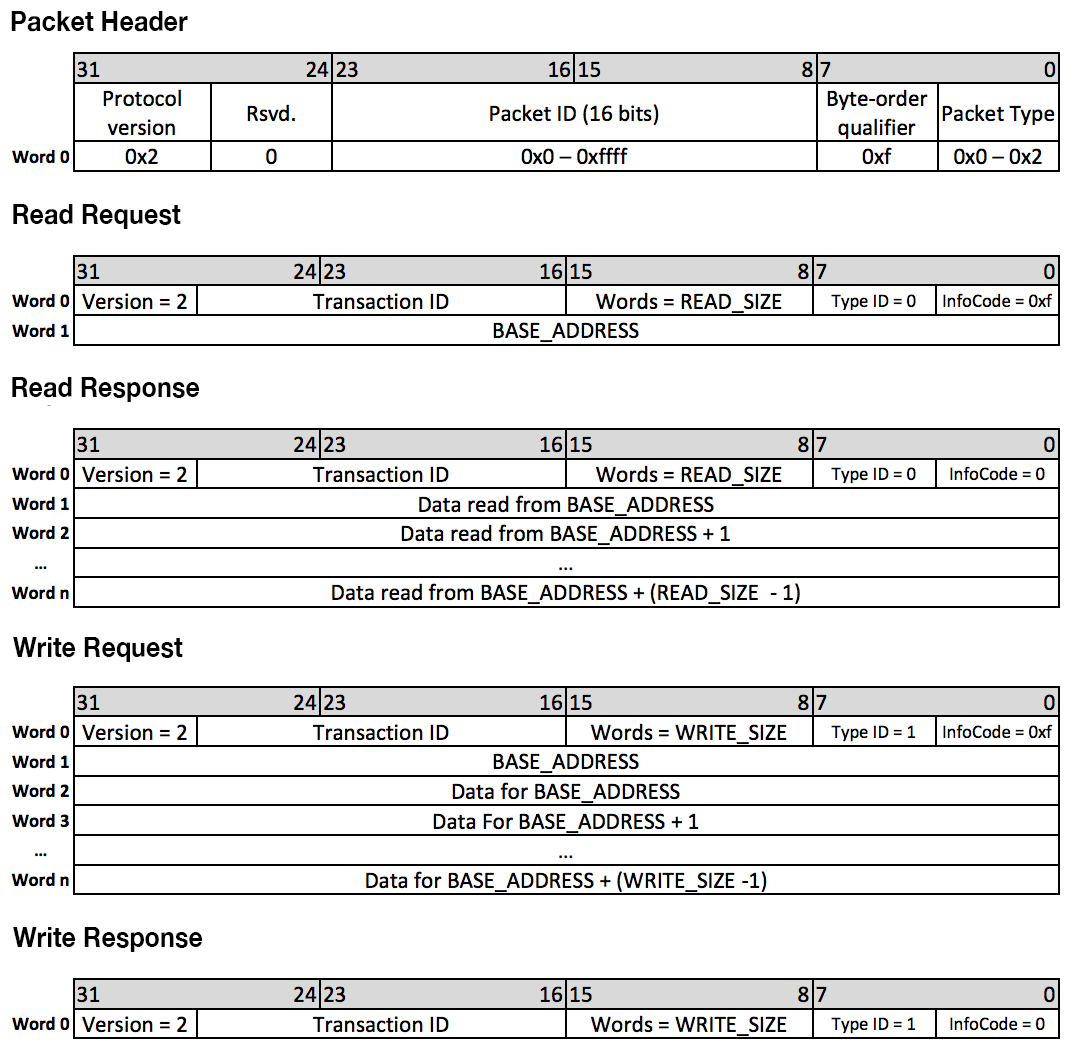
\includegraphics[width=\textwidth]{img/II-2-daq/ipbus.png}
        \caption{??? \cite{AMC13}.}
        \label{fig:II-2-daq-ipbus}
      \end{figure}

      On the electronics side, the IPBus protocol is handled by a master which decodes the requests and forwards it to slaves which each respond to a given address range. Requests involving multiple reads are writes are decomposed by the master in single operations. Slaves receive the request type, address, and data as input parameters and can then treat it as they like. In return, they provide an acknownledgment and optionnally data in the case of a read operation. Eventhough the software treats the address space of 32 bits as a set of read/write registers of 32 bits (A32/D32), the physical implementation on the electronics can be different. Requests can be connected to registers of be used to activate functions on the PCBs. The implementation is up to the developpers.

  \section{The First Prototype of the Data Acquisition System}

    Due to the ongoing developments on the VFAT3 ASIC and the GBT chipset, and to test the feasability of the manufacturing of the GEB, a first prototype of the GE1/1 DAQ system was developped in 2014 with slightly different components. The differences with the final system are shown in Figure \ref{fig:II-2-daq-gem-system-v1} where elements in red are not yet implemented and those in blue are prototypes or variations of the final electronics. The system was composed of six VFAT2 front-end chips, predecessor of the VFAT3, a first prototype of the GEB with only 6 out of the 24 positions active, and a first version of the OptoHybrid optically connected to the GLIB AMC serving as readout board. The usability of the system was tested during a test beam campaign in 2014-2015 which acted as proof of concept for the DAQ system architecture.

    \begin{figure}[h!]
      \centering
      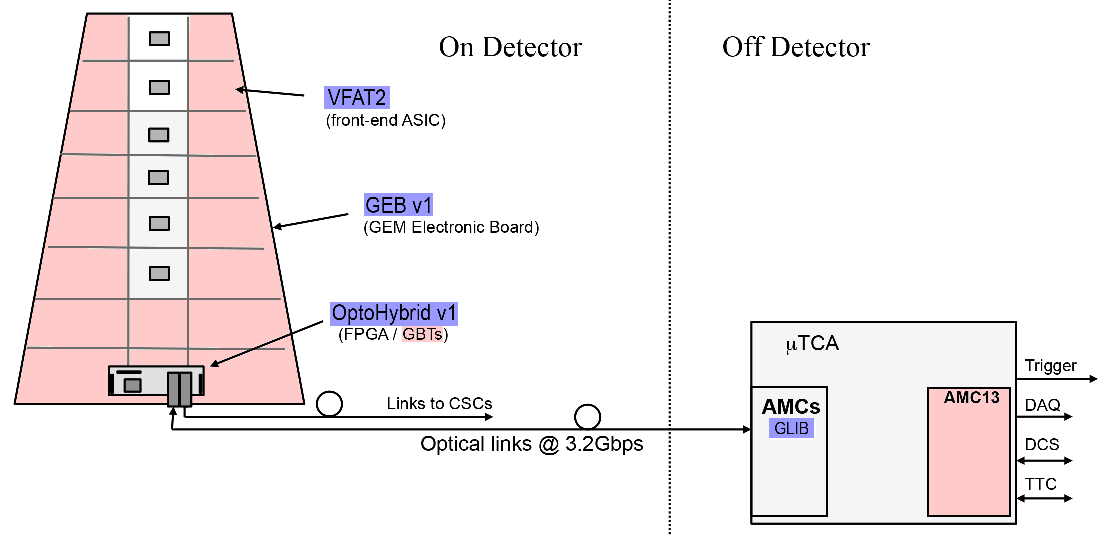
\includegraphics[width=0.9\textwidth]{img/II-2-daq/gem-system-v1.pdf}
      \caption{???.}
      \label{fig:II-2-daq-gem-system-v1}
    \end{figure}

    \subsection{The VFAT2 ASIC}

      Similarly to the VFAT3 ASIC, which architecture has been presented before, the VFAT2 is a binary front-end chip used to digitize signals generated by gaseous detectors. A schematic representation of the chip is depicted in Figure \ref{fig:II-2-daq-vfat2}. The 128 analog signals are preamplified, shaped, and discriminated against a settable threshold in the analog front-end which is asyncrhonous from the LHC clock. Synchronicity is achieved through monostables connected to each channel which allow to generate a binary pulse each time the threshold is reached in a given BX. Moreover, the duration of the output signal of the monostable can be stretched to cover multiple clock cycles. This function is only used in the tracking data stored in the SRAM1 and not the 8 trigger bits, called SBits, formatted by the Trigger unit. Upon reception of a L1A, data is transfered from the SRAM1 to the SRAM2 and serially transmitted over the DataOut and DataValid lines. The DataValid line caries the 192 bits that form an event while the DataOut line signals the validity of the data by going to a logic '1' during transmission. The four fast commands (L1A, Resync, CalPulse, and BC0), called the T1 in the VFAT2 context, are received over a single differential pair and are encoded on three bits meaning that no two consecutive L1As can be received within three BXs. Finally, the configuration of the ASIC is done using the I2C protocol. \\

      \begin{figure}[h!]
        \centering
        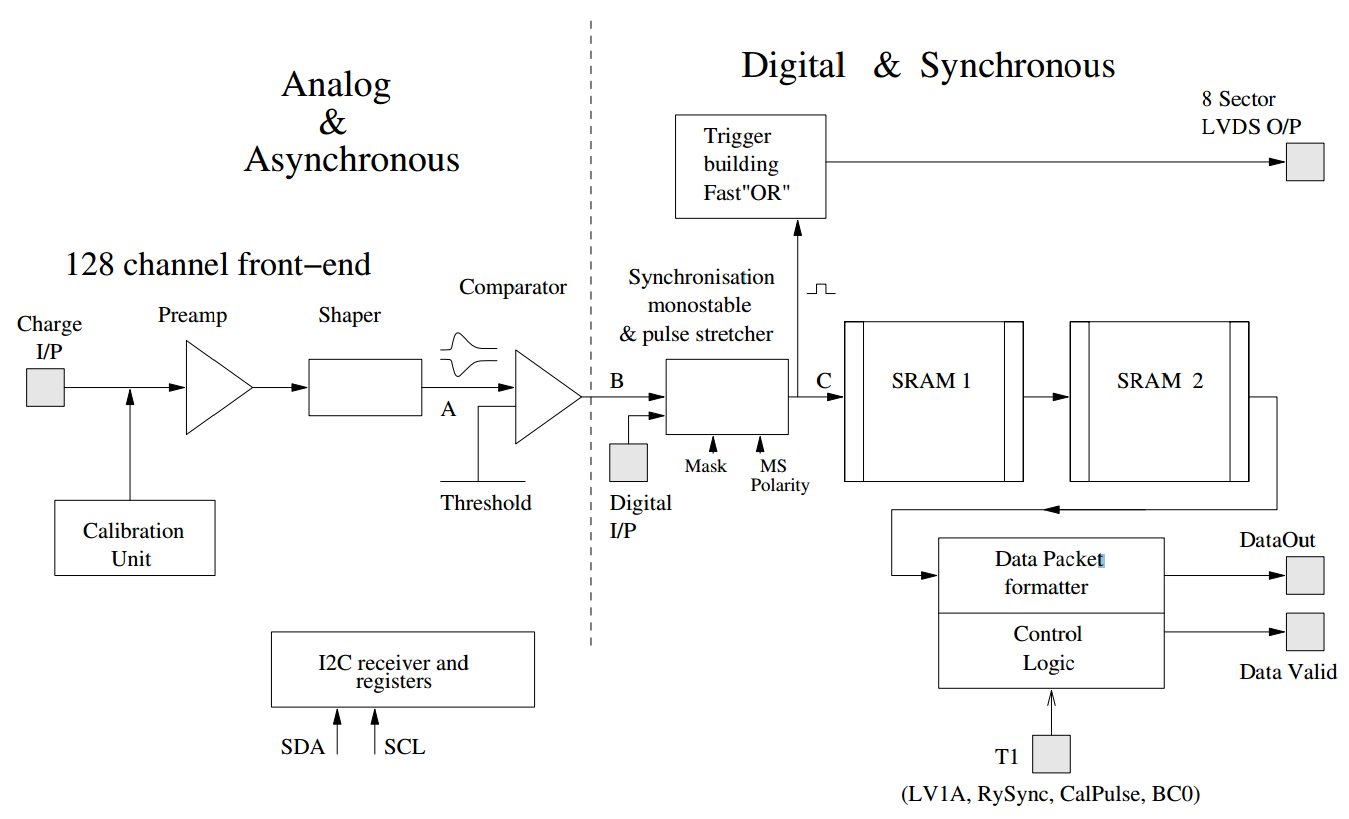
\includegraphics[width=\textwidth]{img/II-2-daq/vfat2.png}
        \caption{??? \cite{Aspell:1069906}.}
        \label{fig:II-2-daq-vfat2}
      \end{figure}

      The main differences between VFAT2 and VFAT3 are the communication protocols and the reduced bandwidth allocated to trigger data over the fixed latency path. While VFAT3 can be directly connect to the GBT chipset, the VFAT2 has to be controlled and readout by the FPGA located on the FPGA. Furthermore, VFAT3 has a trigger granularity of 64 bits per BX while VFAT2 is limited to 8 bits per BX. Altought the configuration of the bits can be chosen through programmable registers, it is common to divide the 128 strips in 8 groups of 16 neighbouring strips and transmit one bit for each group. \\

      As the VFAT2 ASIC does not come within a package like standard ICs, it is bounded to a small PCB called the VFAT2 Hybrid depicted in Figure \ref{fig:II-2-daq-vfat2-hybrid}. The Hybrids are equipped with two connectors: one for the 128 analog input channels and one for the digital signals and the power. They are respectivly connected to the GEM readout plane on one side and the GEB on the other side.

      \begin{figure}[h!]
        \centering
        
\includegraphics[width=\textwidth]{img/empty.png}
        \caption{VFAT2-HYBRID.}
        \label{fig:II-2-daq-vfat2-hybrid}
      \end{figure}

    \subsection{The GEM Electronic Board v1}

      Due to the manufacturing challenge that is the production of a 1-m-long PCB, a first version of the GEB has been produced with minimal features. The first prototype was equipped with only six functionning positions in the middle row closest to the small side of the board. The positions shared a common clock and trigger line and were divided into two slow control sectors. As fewer connections were needed between the GEB and the OptoHybrid, a smaller connector was also used.

    \subsection{The OptoHybrid v1}

      Mounted on the GEB v1 is the OptoHybrid v1, a first prototype designed to demonstrate the concept of an FPGA-based concentrator board to make the communication with the back-end electronics. The OptoHybrid v1, shown in Figure \ref{fig:II-2-daq-ohv1}, is equipped with a Xilinx Spartan-6 FPGA that concentrates the data from the six VFAT2 Hybrids and transmits it over four optical links to the off-detector electronics. It is further equipped with a MSP430 EZ430-RF2500 \cite{MSP430} microcontroller which is used as Analog-to-Digital Converter (ADC) to digitize the analog outputs of the calibration units of the VFAT2s, and some General Purpose Input/Output pins (GPIOs) for debugging.

      \begin{figure}[h!]
        \centering
        
\includegraphics[width=\textwidth]{img/empty.png}
        \caption{OptoHybrid V1.}
        \label{fig:II-2-daq-ohv1}
      \end{figure}

    \subsection{The GLIB Advanced Mezzanine Card}

      Designed by CERN, the Gigabit Link Interface Board (GLIB) \cite{Vichoudis:1359270} has been developped as an evaluation platform for the GBT-FPGA project. As shown in Figure \ref{fig:II-2-daq-glib}, it is a general purpose microTCA AMC equipped with a Xilinx Virtex-6 FPGA, four SFP optical cages, and two extension header that can accomodate custom electronics. The GLIB can be used within the microTCA crate in so called crate-mode, or as standalone board in bench-top mode. To this end, it is equipped with an Ethernet connector to replace the fabric A line coming from the MCHs while still providing access using IPBus. \\

      \begin{figure}[h!]
        \centering
        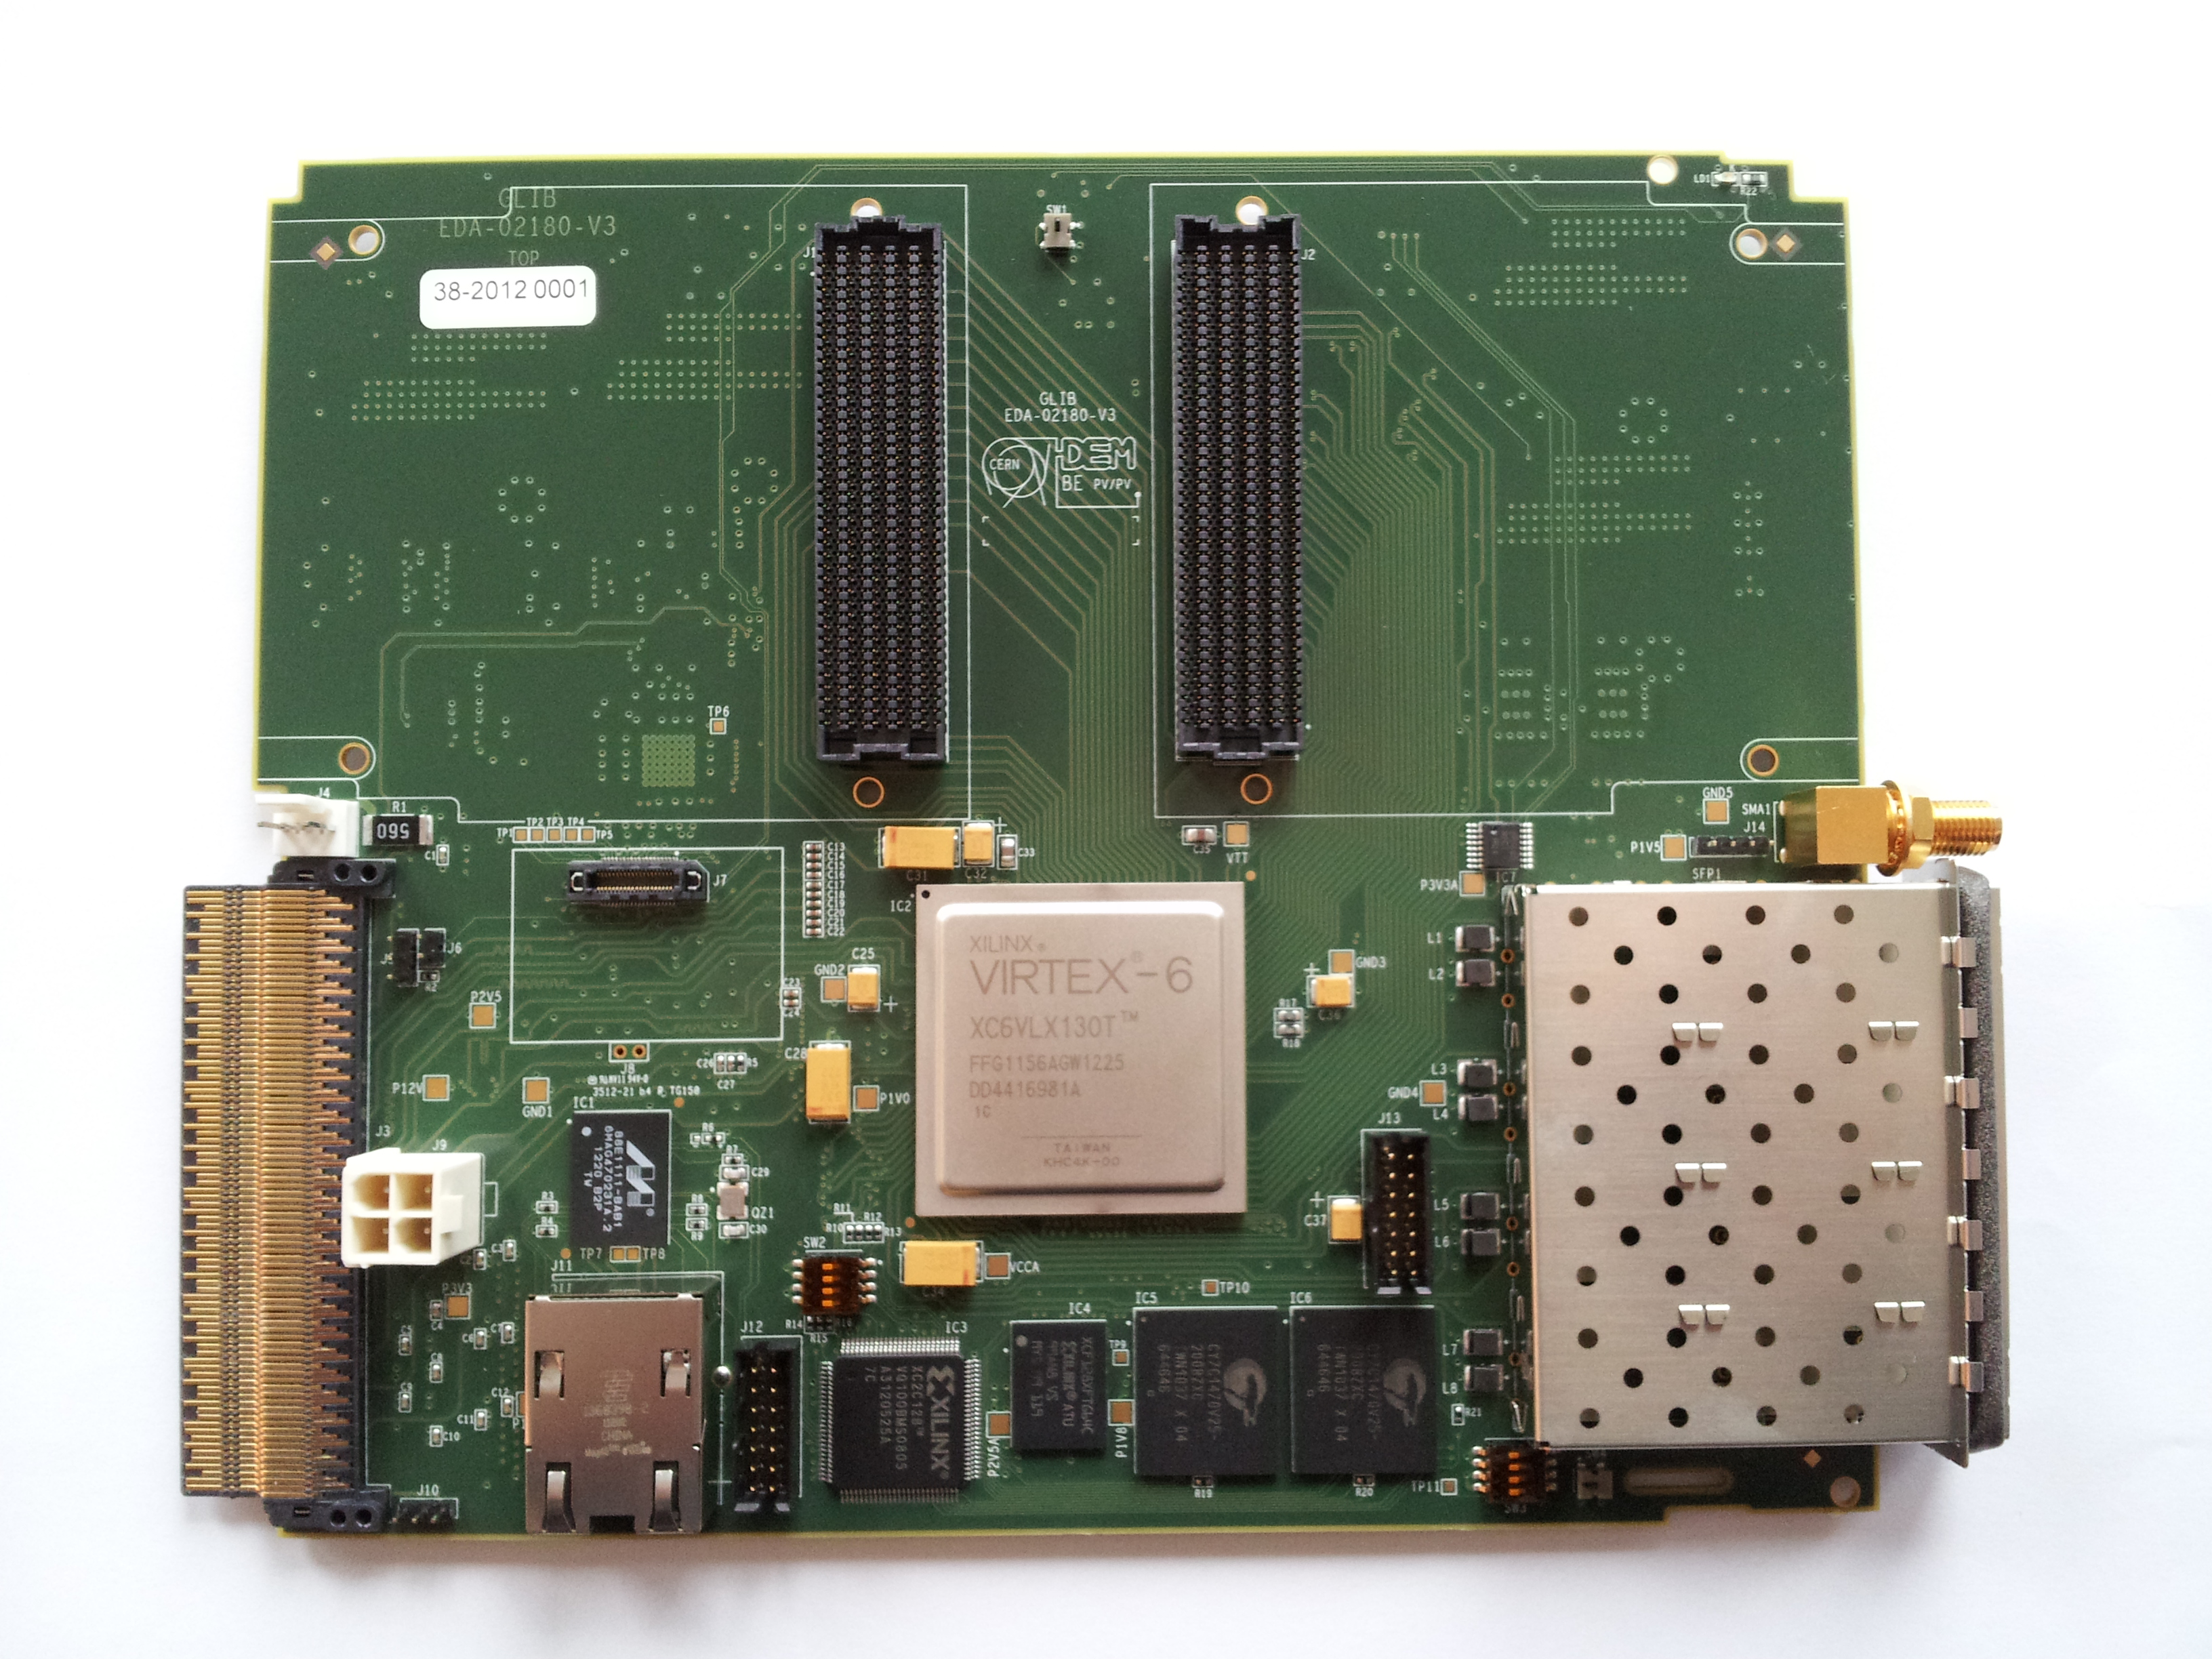
\includegraphics[width=0.8\textwidth]{img/II-2-daq/glib.jpg}
        \caption{\cite{Vichoudis:1359270}.}
        \label{fig:II-2-daq-glib}
      \end{figure}

       In this prototype version, the board has been used as concentrator for the data pushed by the OptoHybrid which is stored locally and then pulled by the monitoring application over IPBus. The slow control requests were also handles directly by the GLIB over IPBus and forwarded to the OptoHybrid.

  \section{The GE1/1 Data Acquisition System for the Test Beam}

    Incrementing on the first prototype developped in 2014, a second version of the system has been developped in 2015 and tested during test beams in November of the same year and which results are exposed in Chapter \ref{chap:II-3-test-beam}. This system, shown in Figure \ref{fig:II-2-daq-gem-system-v2a}, has many similarities with the first prototype, only increasing the number of supported VFAT2 Hybrids to 24 which, however, required a complete redesign of the GEB and the OptoHybrid. The back-end system is still handled by the GLIB board which is controlled and readout through IPBus.

    \begin{figure}[h!]
      \centering
      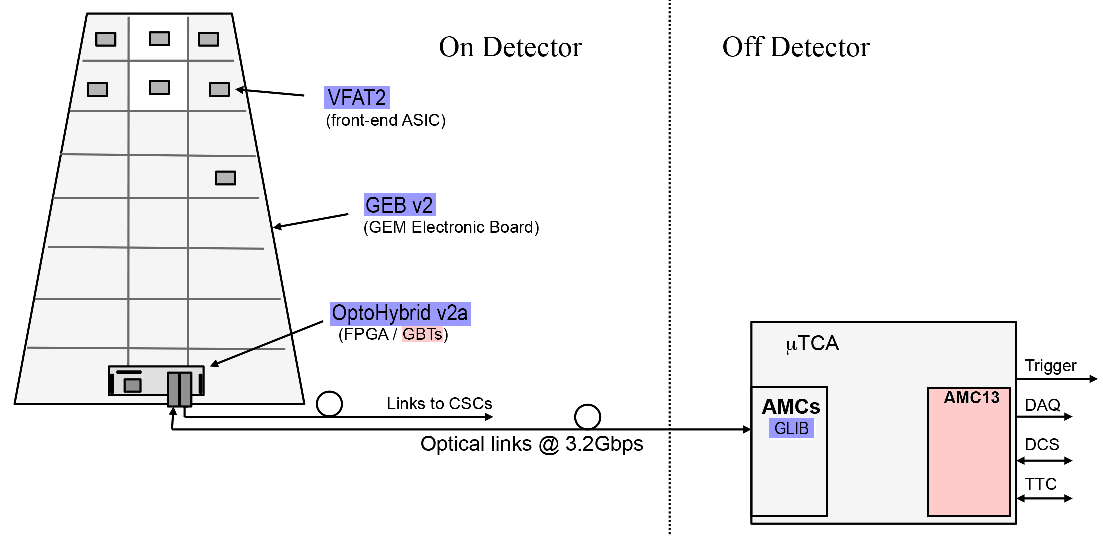
\includegraphics[width=0.9\textwidth]{img/II-2-daq/gem-system-v2a.pdf}
      \caption{???.}
      \label{fig:II-2-daq-gem-system-v2a}
    \end{figure}

    \subsection{The GEM Electronic Board v2}

      The GEB v2 handles 24 VFAT2 Hybrids divided in three columns for the clock and fast control distribution, and six sectors for the slow control I2C protocol. The connection to the OptoHybrid is done through four connector that transmit the trigger, tracking, and command signals from the VFAT2s to the FPGA.

    \subsection{The OptoHybrid v2a}

      The second version of the OptoHybrid is still a prototyping board which offers various configuration schemes to select the best operating mode. Represented in Figure \ref{fig:II-2-daq-ohv2a}, the OptoHybridv2a uses a Xilinx Virtex-6 FPGA similar to the GLIB. It can either use 12 SFP optical cages or a QSFP+ transceiver which offers four optical connections in a single module. The LHC clock can be recovered by the Texas Instrument CDCE62005 which is a programmable clock generator or by the radiation hard QPLL module developped by CERN specifficaly to this end.

      \begin{figure}[h!]
        \centering
        
\includegraphics[width=\textwidth]{img/empty.png}
        \caption{OptoHybrid V2a.}
        \label{fig:II-2-daq-ohv2a}
      \end{figure}

  \section{The GE1/1 Data Acquisition System for the Slice Test}

    The last prototype of the architecture before developments for the final system start is the DAQ system for the slice test which is to be installed in January 2017. The architecture of the system is depicted in Figure \ref{fig:II-2-daq-gem-system-v2b}. Altough this small scale test will be performed using the VFAT2 ASIC as the VFAT3 is still in developments, other components are more similar to the final version. The GBT chipset, which production has started, is used along with a more powerful microTCA AMC very similar to the MP7. Readout is performed using the AMC13 connected to the central DAQ of CMS.

    \begin{figure}[h!]
      \centering
      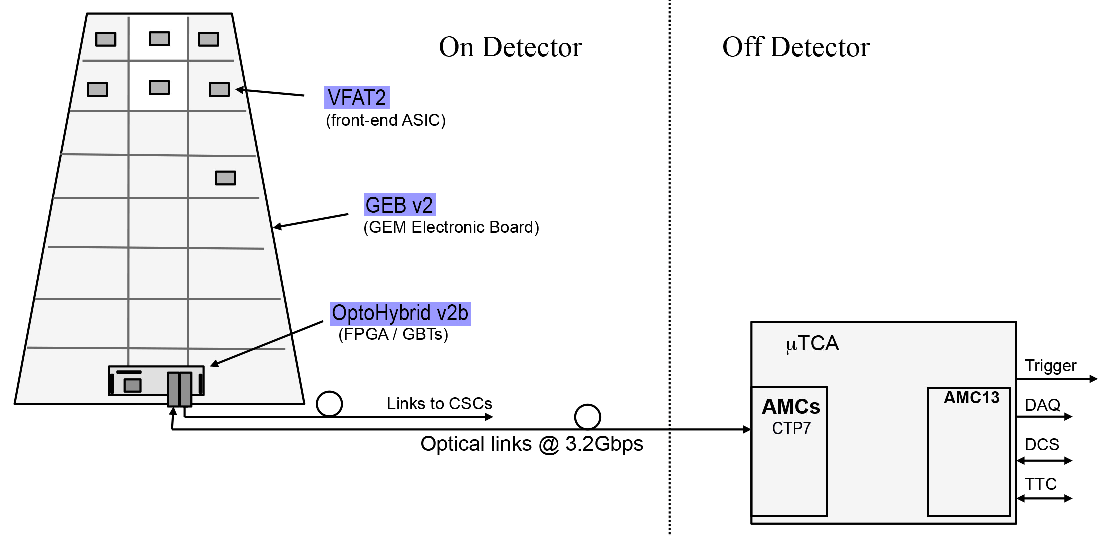
\includegraphics[width=0.9\textwidth]{img/II-2-daq/gem-system-v2b.pdf}
      \caption{???.}
      \label{fig:II-2-daq-gem-system-v2b}
    \end{figure}

    \subsection{The OptoHybrid v2b}

      The second iteration on the OptoHybridv2 has a U shape to accomodate the constraints of the detector geometry, cooling system, and front-pannel as shown in Figure \ref{fig:II-2-daq-ohv2b}. It is equipped with four optical links using the SFP cages and the VTRx and VTTx modules. Three of the links are controlled by the FPGA itsel while the last one is connected to a GBT chipset in turn controlled by the FPGA. The QPLL has been chosen over the CDCE62005 for its simplicity of use and its tolerance to radiation. The connection to the GEB and the GEB itsel remain unchanged.

      \begin{figure}[h!]
        \centering
        
\includegraphics[width=\textwidth]{img/empty.png}
        \caption{OptoHybrid V2b.}
        \label{fig:II-2-daq-ohv2b}
      \end{figure}

    \subsection{The CTP7 AMC}

      \begin{figure}[h!]
        \centering
        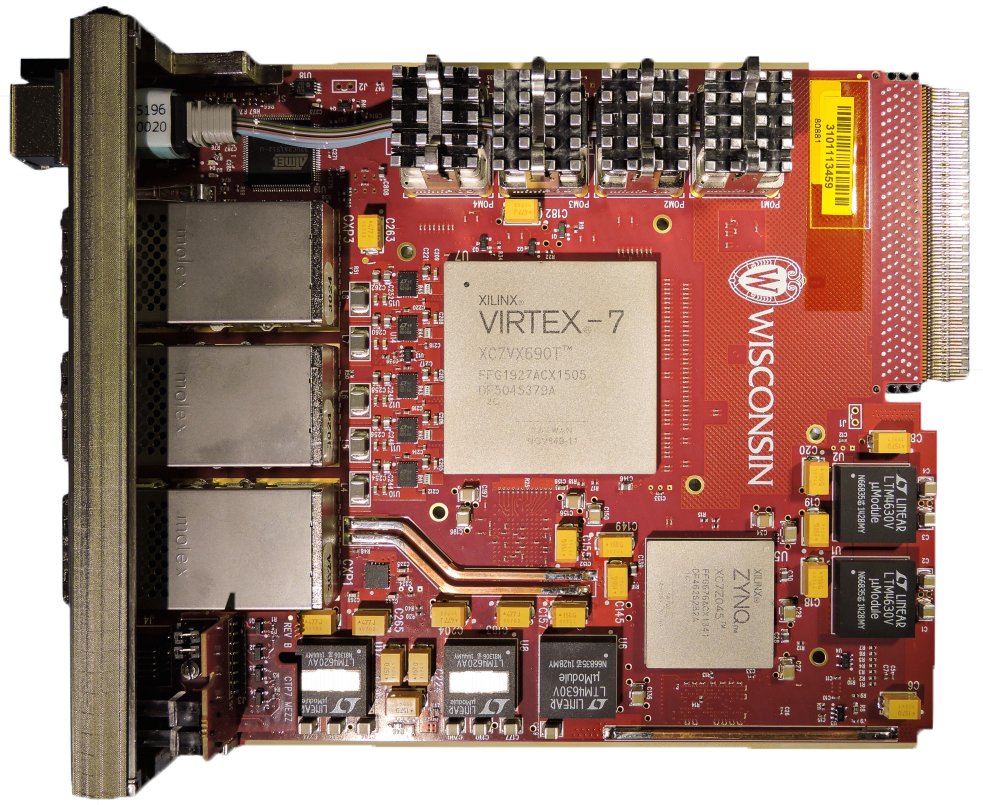
\includegraphics[width=0.8\textwidth]{img/II-2-daq/ctp7.png}
        \caption{OptoHybrid V2b.}
        \label{fig:II-2-daq-ctp7}
      \end{figure}

  \section{Summary}

    To summarize the evolution of the DAQ system and the various components used

    \begin{table}
      \begin{tabularx}{\textwidth}{C{1}C{1}C{1}C{1}}
        \textbf{First prototype} & \textbf{Test beam}   & \textbf{Slice test}  & \textbf{Final system} \\ \hline
        6x VFAT2        & 24x VFAT2   & 24x VFAT2   & 24x VFAT3 \\
        GEB v1          & GEB v2      & GEB v2      & GEB v3 \\
        OptoHybrid v1           & OptoHybrid v2a      & OptoHybrid v2b      & OptoHybrid v3 \\
        -               & -           & 1x GBT      & 3x GBT \\
        GLIB            & GLIB        & CTP7        & MP7 \\
        -               & -           & AMC13       & AMC13 \\
      \end{tabularx}
      \caption{??}
    \end{table}
































-
